%Document Class
\documentclass[a4paper, 10pt]{IEEEtran}

%Packages
\usepackage{bm} %this package gives bold maths text with command \bm{<>}
\usepackage{graphicx} %graphics package for adding images/figures
	\graphicspath{{images/}} %the path for graphicx to retrieve the images
\usepackage{float} %adds the image positioning parameter `H'
\usepackage{amsmath, amssymb} %adds a wide range of maths symbols and functions
\usepackage{gensymb} %more maths symbols
\usepackage{stfloats} %better handling of `b' position for double column figures etc.

\usepackage{textcomp} %this package is only used to create the superscript 'st' in the title

%Document
\begin{document}

%Title Section
\title{Decision Making in a Committee}
\author{Hayk Khachatryan}
\maketitle

%Running Header
\markboth{Department of Physics and Astronomy, UCL. \today}{E., Armadillo: Nihilism in the 21st Century}

\begin{abstract}
This paper was produced with absolutely no prior research. The data is completely made up and bears very little relevance to the paper's title or the work conducted. Consequently any conclusions that might be made are wholly invalid. Nonetheless the findings of this paper indicate that the popularity of nihilistic thought grew  steadily over the course of the 20th Century. That growth has been accelerated in the last $\bm{13 \pm 2}$ yrs by the introduction of social media and `memes'.
\end{abstract}

\begin{IEEEkeywords}
Nihilism, Social Media, Social Behaviour.
\end{IEEEkeywords}



\section{Introduction}
\label{sec:introduction} %label this section `sec:introduction' so it can be referred to

\subsection{Background}
\label{sec:background}

\IEEEPARstart{T}{he} %drop cap the first word
term `nihilism' was first coined by German philosopher Friedrich Heinrich Jacobi. It's rise in popularity during the mid-19th Century can be ascribed in part to the Russian novelist Ivan Turgenev. In it's earliest form, nihilistic philosophy described the act of suppressing one's individualism; reducing it to a non-existent, meaningless entity. Many of the individuals who first posited the idea of nihilism advocated strongly against it, believing instead that it was better to maintain a faith in God. \par

In the 19th Century `nihilistic beliefs' led to a life without meaning, worth or value. Meanwhile, modern nihilism contends that there is nothing of meaning, worth or value to begin with. This subtle shift in the definition of the term may be, in-part, due to the work of German philosopher Friedrich Nietzsche, who wrote about nihilism as a widespread phenomenon within Western culture. Nietzsche used the notion of nihilism throughout his work, but often with a variety of connotations. An underlying theme is that nihilism involves, to some extent, the loss of morality and the idea that meaning is something we attribute ourselves. \cite{WikNi}%reference the citation labelled `WikNi' 
\par

In a Christian society this appeared to run counter to the notion that meaning and purpose were ascribed by God. This paper\footnote{Under no means should this be interpreted as an exemplar paper. It is merely intended as a template and your own work should in no way reflect the quality of content herein.} looks at whether, in a more secular 21st Century society, the advent of social media as led to a growth in nihilistic beliefs.

\section{Method}
\label{sec:method}

The method was long and complicated, it involved months of meticulous planning and preparation. It was exacted in four steps, which are detailed below.

\subsection{Graphing}
\label{sub:graphing}


\subsubsection{Creating the graph}
\label{subsub:creation}

The first step was to create a cyclic graph with $n$ nodes, each connected to their $k$ nearest neighbors. The nodes were randomly assigned binary opinions of $1$ or $0$, see Fig \ref{fig:graphing}(a), then the links between neighbors were randomly rewired with probability $e$, as can be seen in Fig \ref{fig:graphing}(b). The resultant structure and connections of the graph remained constant throughout the rest of the process.\par

\begin{figure}[H]
\centering
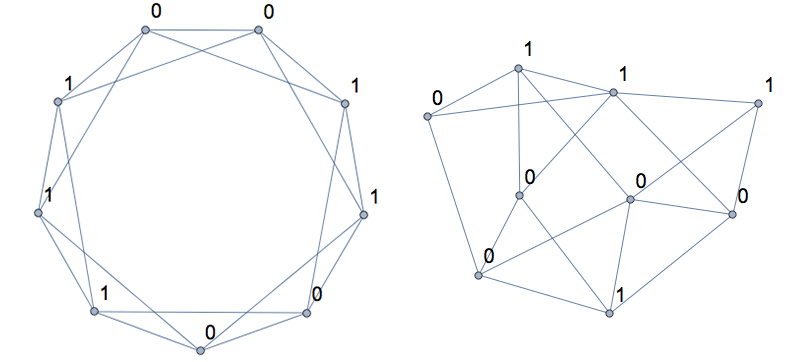
\includegraphics[width=\linewidth]{graphs.png}
\caption{(a) A graph with $n = 9$, $k = 4$ and (b) a graph with the same parameters but rewired with probability $e = 0.1$.}
\label{fig:graphing}
\end{figure}

\subsubsection{Paths}
\label{subsub:paths}

An update was carried out random-sequentially through the nodes, ie in each iteration a random path across the nodes was chosen and the states of each node were updated sequentially using a majority rule. Once all of the nodes had been updated (once each), a new random path was assigned and the nodes were once again updated, see Table \ref{tab:paths} below for an example. Updates were carried out dynamically: within an iteration node states were called as their neighbor was reached in the path, not once at the beginning; ie if node $5$'s state was changed to $1$ from $0$, the new state ($1$) is used for subsequent calculations involving node $5$ in the same iteration.

\begin{center} %centers table and caption in column
	\begin{minipage}{.7\linewidth} %use a minipage to compress the table caption
	\begin{table}[H]
		\centering %center the table within the minipage
		\renewcommand{\arraystretch}{1.3} %change \arraystretch in `tabular' to increase row height
		\caption{An example of random-sequential paths.}
		\label{tab:paths}
		\begin{tabular}{c | c} %two centered columns, separated by a vertical line
			Iteration & Path across nodes (nodes labelled numerically) \\ \hline \hline %double horizontal line
			1 & 3 $\rightarrow$ 1 $\rightarrow$ 9 $\rightarrow$ 5 $\rightarrow$ 6 $\rightarrow$ 2 $\rightarrow$ 8 $\rightarrow$ 7 $\rightarrow$ 4 \\ \hline
			2 & 5 $\rightarrow$ 3 $\rightarrow$ 9 $\rightarrow$ 7 $\rightarrow$ 8 $\rightarrow$ 4 $\rightarrow$ 2 $\rightarrow$ 6 $\rightarrow$ 1 \\ \hline
			3 & 7 $\rightarrow$ 5 $\rightarrow$ 4 $\rightarrow$ 1 $\rightarrow$ 8 $\rightarrow$ 6 $\rightarrow$ 9 $\rightarrow$ 3 $\rightarrow$ 2 \\ \hline
		\end{tabular}
	\end{table}
	\end{minipage}
\end{center}


\subsubsection{Majority Rule}
\label{subsub:majority}

The state of each node was updated using a majority rule with a threshold, $h \in [0.5, 1]$. A majority above the threshold, $h$, was required for the state of a node to be updated. See Table \ref{tab:majority} below.

\begin{center} %centers table and caption in column
	\begin{minipage}{.7\linewidth} %use a minipage to compress the table caption
	\begin{table}[H]
		\centering %center the table within the minipage
		\renewcommand{\arraystretch}{1.3} %change \arraystretch in `tabular' to increase row height
		\caption{An example of the majority rule with $h = 0.6$.}
		\label{tab:majority}
		\begin{tabular}{c | c | c} %three centered columns, separated by a vertical line
			Node value & Connected node values & New node value\\ \hline \hline %double horizontal line
			0 & 0, 0, 0, 1, 1 & 0 \\ \hline
			0 & 0, 0, 1, 1, 1 & 1 \\ \hline
			1 & 0, 0, 0, 1, 1 & 0 \\ \hline
		\end{tabular}
	\end{table}
	\end{minipage}
\end{center}


\subsection{Dissensus}
\label{sub:dissensus}

Dissensus was measured with using the committee size and  the final population with state $0$, across all possible values of the initial population with  state $0$.  This gives

\begin{align}
\label{eq:dissensus}
D(N) \equiv \Biggl\langle \Theta \Biggl(1 - \frac{max(S_f, N - S_f)}{N}\Biggr)\Biggr \rangle_{S_i}
\end{align}

where $N$ is the committee size, $S_f$ the final population with  state $0$, $S_i$ the initial population with state $0$, $\langle \cdot \rangle_{S_i}$ the mean across all possible values of $S_i$, and $\Theta (x)$ the Heaviside step function ($0$ for $x = 0$ and $1$ for $x > 0$). 

\begin{align}
\label{eq:intrest}
\begin{split}
	\frac{\partial y}{\partial x} &\simeq \int_{-1}^{1} { \frac{3x}{2} }^{ -\infty } + \pi \quad dx \\ %quad is a spacing command to separate the dx from integral
	&= \left[ \frac{ 3x^ { 1 - \infty } }{ 2 ( 1 - \infty ) } + \{ \pi \cdot x \} \right] ^{1}_{-1} \\
	&= 0
\end{split} \\[10pt]
\therefore \; y &\approx 0 %\; is a spacing command to separate the `therefore'
\end{align}

Since we also have:

\[
y = mx + c
\]

We know that the first stage of the method was thus inconclusive. In order to understand why, it was necessary to develop a second stage.

\subsection{Data Collection}
\label{sub:datacollection}

No data was collected, instead table \ref{tab:armadillo}, %reference the table labelled `tab:armadillo'
detailing the anatomy of an armadillo, has been included. It contains ranges for the dimensions of known armadillo species, from the chipmunk-sized, pink fairy armadillo to the largest species - the giant armadillo \cite{WikAr}.

\begin{center} %centers table and caption in column
	\begin{minipage}{.7\linewidth} %use a minipage to compress the table caption
	\begin{table}[H]
		\centering %center the table within the minipage
		\renewcommand{\arraystretch}{1.3} %change \arraystretch in `tabular' to increase row height
		\caption{A table illustrating the range of dimensions for different armadillo species.}
		\label{tab:armadillo}
		\begin{tabular}{c | c} %two centered columns, separated by a vertical line
			Dimension & Value \\ \hline \hline %double horizontal line
			Mass (kg) & 0.085 - 54 \\ \hline
			Length (cm) & 13 - 150 \\ \hline
			Body Temp (\textdegree C) & 33-36 \\ \hline
		\end{tabular}
	\end{table}
	\end{minipage}
\end{center}

\section{Results and Analysis}
\label{sec:resultsanalysis}

The results of this study indicate that, throughout the course of the 20th Century, the concept of nihilism underwent a substantial development. Movement from the fringes to a more mainstream ideology resulted in a noticeable re-definition of the term. The ideas of Nietzsche were notably adopted by Heidigger who recognised nihilism as an attempt to achieve some moral victory through the deprication of common values \cite{WikMH}. \par

Heidigger felt that 20th Century Western culture teetered on the brink of total nihilism, and that a new technological age presented society with two possible paths: the end of metaphysics and modernity; or a type salvation. He believed that the former would, ironically, be celebrated as a new age of enlightenment. It is within this context that the rise of internet pages promoting nihilism, and the increasing popularity of `nihilistic memes' are particularly interesting. \par

The proliferation of `nihilistic' memes and the ease with which anyone is able to create them has resulted, to some extent, in a loss of meaning to the term. To an increasing extent \cite{npec1}, `nihilism' has become an umbrella term; used to represent the concepts of pessimism, egoism and cynicism - the distinctions between which have been somewhat muddied. Perhaps this is symptomatic of the `enlightenment' Heidigger foresaw.

\begin{figure*}[b] %`starred' figure environment allows two column image
\label{fig:usage}
\centering
\begin{minipage}{.8\linewidth} %minipage to reduce caption width
	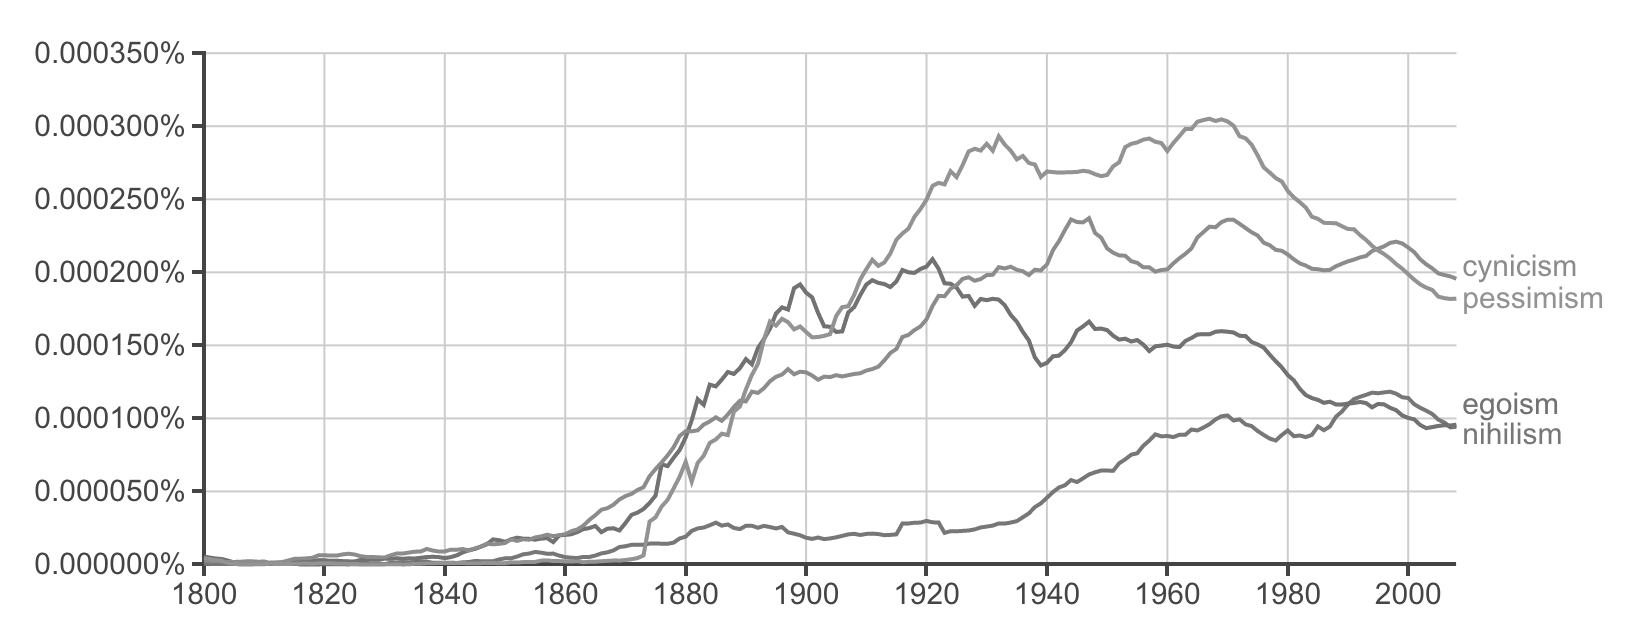
\includegraphics[width=\linewidth]{usage.png}
	\caption{A steady, post-war, increase in the prevelance of the term `nihilism' is mirrored by a steady decline in the usages of `pessimism', `egoism' and `cynicism'.}
\end{minipage}
\end{figure*}

Social media networks allow individuals to propagate beliefs and ideologies, often through content known as a `meme', which is usually composed of a satirical or humorous image and a short piece of text that often conveys and emotion, thought or action. Social media pages devoted to publishing memes will often generate several a day, through user submissions or by developing original content.

Work published by `nihilistic' meme pages is often unverified and thus often created by non-specialist individuals with no formal education in the subject, and for whom the study of nihilism as a philosophy consists of little more than following other `nihilistic' social media accounts, as shown in equation (\ref{eq:matrix}).

\begin{align}
\label{eq:matrix}
A &=
\begin{pmatrix}
	e^m & 0 \\
	-1 & me^{}
\end{pmatrix} \\[1pt]
B &=
\begin{pmatrix}
	me^{} & 0 \\
	1 & e^m
\end{pmatrix} \\[10pt]
\therefore \; A \cdot B &=
\begin{pmatrix}
	me^{m}e^{} & 0 \\
	0 & me^{m}e^{}
\end{pmatrix}
\end{align}

\vspace{0.5em} %add extra blank vertical space below matrix

\section{Conclusion}
\label{sec:conclusion}

In conclusion, this template contains examples of some of the key features that might be found in a formal report created using \LaTeX. One more thing that's needed however is a list of armadillo species:

\begin{itemize} %start list
\item Banded Armadillos
\begin{enumerate} %start sub-list
	\item Seven-Banded
	\item Nine-Banded
\end{enumerate}
\item Airy Armadillos
\begin{itemize}
	\item Fairy Armadillos
	\begin{itemize}
		\item Greater Fairy
		\item Pink Fairy
	\end{itemize}
\end{itemize}
\end{itemize}

As you can see, there are lots of species of armadillo, some of which are nihilistic, but all of which are highly existential.

\begin{thebibliography}{99}
\label{references}

\bibitem{WikNi}
	R. L. Myer, ``Parametric oscillators and nonlinear materials,'' in \textit{Nonlinear Optics}, vol. 4, P. G. Harper and B. S. Wherret, Eds. San Francisco, CA: Academic, 1977, pp. 47-160.

\bibitem{WikAr}
	E. E. Reber et al., ``Oxygen absorption in the earth’s atmosphere,'' Aerospace Corp., Los Angeles, CA, Tech. Rep. Angeles, CA, Tech. Rep. TR-0200 (4230-46)-3, Nov. 1988.

\bibitem{WikMH}
	J. Jones. (1991, May 10). \textit{Networks} (2nd ed.) [Online]. Available: http://www.atm.com

\bibitem{NGRAM}
	 R. E. Kalman, ``New results in linear filtering and prediction theory,'' \textit{J. Basic Eng.}, ser. D, vol. 83, pp. 95-108, Mar. 1961.

\bibitem{NiMeme}
	J. P. Wilkinson, “Nonlinear resonant circuit devices,” U.S. Patent 3 624 125, July 16, 1990.


\end{thebibliography}

\end{document}